\documentclass[a4paper,10pt]{article}

\usepackage[utf8x]{inputenc}
\usepackage[slovene]{babel}
\usepackage{amsmath}
\usepackage{amsfonts}
\usepackage{relsize}
\usepackage[smaller]{acronym}
\usepackage{graphicx}
\usepackage{subfigure}
\usepackage{cite}
\usepackage{url}
\usepackage{hyperref}
\usepackage{color}
\usepackage[version=3]{mhchem}
\usepackage{wrapfig}

%opening
\title{Hidrodinamske nestabilnosti}

\renewcommand{\vec}{\mathbf}

\begin{document}
\begin{center}

\includegraphics[width=6cm]{../logo_fmf_uni-lj_sl}\\[0.5cm]
Oddelek za fiziko \\[2cm]
{ \large Seminar -- 1. letnik, II. stopnja } \\[1cm]
{ \huge \bf Hidrodinamske Nestabilnosti}\\[2cm]
{\large Avtor: Miha \v Can\v cula}\\[0.6cm]
{\large Mentor: prof. dr. Alojz Kodre} \\[0.6cm]
{\large Ljubljana, marec 2012}
\end{center}
\vfill

\begin{abstract}

\end{abstract}

\section{Uvod}

\section{Stabilnost}

O nestabilnosti govorimo, ko infinitezimalno majhna sprememba trenutnega stanja lahko povzro"ci ve"cjo, merljivo razliko po nekem kon"cnem "casu~\cite{drazin}. 

Tak"sna definicija je precej splo"sna, zato jo za potrebe seminarja raje definiramo o"zje in bolj eksaktno: Imejmo sistem, katerega "casovno spreminjanje lahko z eno ali ve"c diferencialnimi ena"cbami, ki imajo dolo"ceno simetrijo. Z nastavkom, ki upo"steva to simetrijo, lahko dobimo re"sitev ena"cb. Stabilnost se poka"ze, ko temu nastavku dodamo majhno motnjo, ki ne upo"steva simetrije. Stabilni sistem se bo vrnil v simetri"cno stanje, medtem ko pri nestabilnem pride do zloma simetrije. 

Primer nestabilnega pojava je svin"cnik, postavljen na konico. Ena"cba, ki opisuje njegovo gibanje, je simetri"cna glede na rotacijo okrog osi svin"cnika. Zato lahko najdemo re"sitev z enako simetrijo, to je pokon"cna lega. "Ce pa svin"cnih le malo izmaknemo iz simetri"cne lege, bo padel in kon"cal v stanju brez rotacijske simetrije. 

\section{Hidrodinamika}

Na nestabilnosti pogosto naletimo pri "studiju curkov teko"cin~\cite{eggers}. 

\section{Tanki filmi}

Hidrodinamsko nestabilnost lahko opazujemo pri polzenju teko"cine po klan"cini~\cite{kondic}. 

\begin{figure}[h]
\centering
 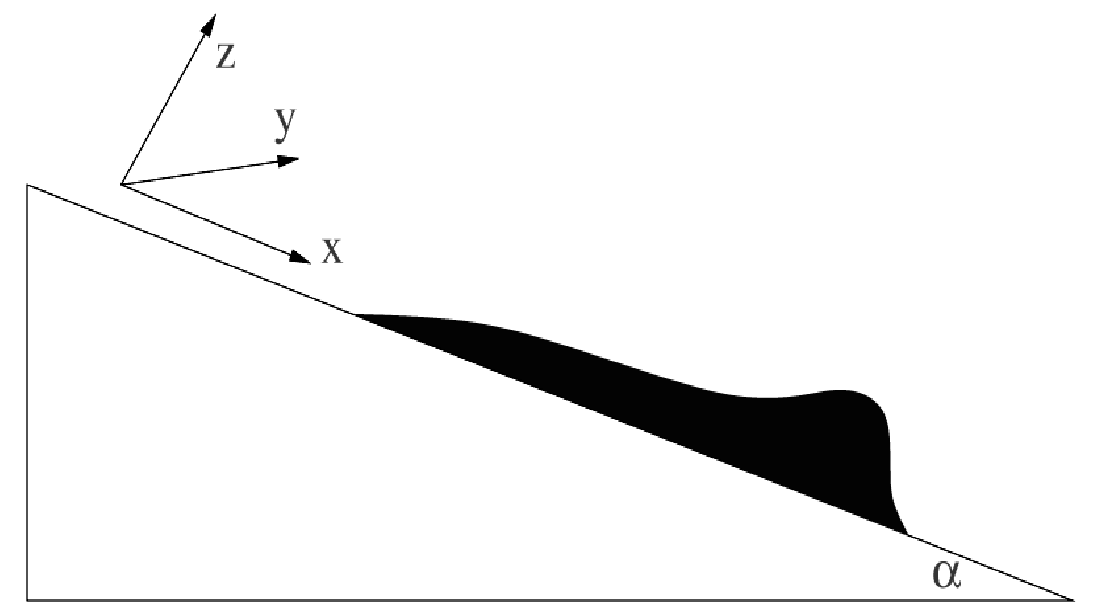
\includegraphics[width=.8\textwidth]{./Slike/film-skica}
\caption{Skica teko"cine v dveh dimenzijah. Viden je greben tik za fronto teko"cine in pa zo"zitev dale"c za fronto, ki je pri ra"cunih ne bomo upo"stevali}
\label{fig:film-skica}
\end{figure}


\subsection{Ena"cbe}

"Ce privzamemo nestisljivost teko"cine $\nabla \cdot \vec u = 0$, se Navier-Stokesova ena"cba poenostavi v 

\begin{align}
 \label{eq:ns-film}
 \frac{\partial \vec u}{\partial t} + (\nabla \cdot \vec u) &= -\frac{1}{\rho}\nabla p + \frac{\mu}{\rho}\nabla^2 \vec u + g (\sin \alpha \vec i - \cos \alpha \vec k)
\end{align}

kjer je $\vec u$ hitrost teko"cine, $\rho$ njena gostota in $\mu$ viskoznost. "Clena z $g$ sta dinami"cna in stati"cna komponenta sile te"ze. Pomembni so tudi robni pogoji, obi"cajno se izbere slede"ce:

\begin{itemize}
 \item Na meji med teko"cino in klancem teko"cina ne drsi, torej je tam $\vec u = 0$. 
 \item Na meji med teko"cino in zrakom ima tlak nezveznost, ki jo sorazmerja povr"sinski napetosti in ukrivljenosti meje $\kappa$. 
\end{itemize}

Ker obravnavamo tanke filme, lahko privzamemo, da je debelina $h$ manj"sa od katerekoli dol"zinske skale v ravnini. S tem privzetkom lahko ena"cbo (\ref{eq:ns-film}) poenostavimo v ena"cbo za $h$. 

\begin{align}
 \frac{\partial h}{\partial t} = -\frac{1}{3\mu}\nabla \cdot \left[ \gamma h^3 \nabla \nabla^2 h - \rho g h^3 \nabla h \cos \alpha + \rho g h^2 \sin \alpha \vec i \right]
\end{align}

\subsection{Brezdimenzijska oblika}

\section{Milni mehur"cki}

Milni mehur"cki so stabilni na majhne motnje zaradi povr"sinske napetosti teko"cine. "Ce pa mehur"cek predremo v eni to"cki, ustvarimo rob, kjer povr"sinska napetost ni uravnote"zena, zato se rob za"cne umikati. Ker je opna obi"cajno zelo tanka, 
je ukrivljenost na robu velika, zato fronta napreduje zelo hitro~\cite{diploma}. To napredovanje je pri mehur"ckih tako hitro, da s prostim o"cesom fronte sploh ne opazimo, ampak se nam zdi, da celoten mehur"cek razpade naenkrat. 
 
\begin{figure}[h]
 \centering
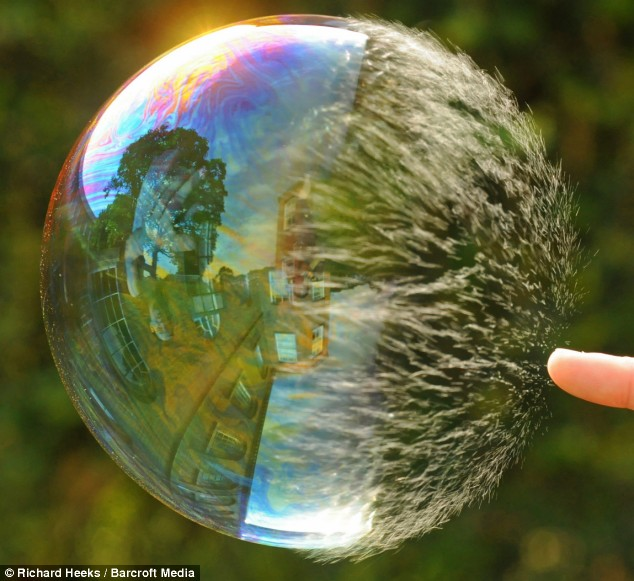
\includegraphics[width=.8\textwidth]{./Slike/bubble-3}
\caption{Razpad milnega mehir"cka~\cite{slike-mehurcek}. Kapljice na desni strani niso posejane enakomerno, ampak so vidni ve"cje in manj"se gostote. }
\end{figure}


\section{Razpad toka v kapljice}

\section{Zaklju"cek}

\begin{thebibliography}{3}
  \bibitem{diploma} S. "Copar, Numeri"cna analiza nestabilnosti na robu teko"cinske opne, Diplomsko delo (2009)
  \bibitem{kondic} L. Kondic, SIAM Review \textbf{45}, 95 (2003)
  \bibitem{eggers} J. Eggers in E. Villermaux, Rep. Prog. Phys. \textbf{71}, 036601 (2008)
  \bibitem{drazin} P. G. Drazin, \textit{Introduction to hydrodynamic stability}, Cambridge University Press (2002)
  \bibitem{slike-mehurcek} \url{http://www.dailymail.co.uk/sciencetech/article-1199149/Super-slow-motion-pictures-soap-bubble-bursting-stunning-detail.html} (23. 1. 2012)
\end{thebibliography}


\end{document}
